\documentclass[final]{beamer}
  \mode<presentation>
  {
% you can chose your theme here:
%  \usetheme{Aachen}
  \usetheme{I6dv}
%  \usetheme{I6pd}
%      \usetheme{Berlin}
%  \usetheme{I6pd2}
%  \usetheme{I6td}
%  \usetheme{Oldi6}
}
% \graphicspath{{figures/}}
% \usepackage[T1]{fontenc}
% Needed for Type1 Concrete
% \usepackage{concrete}

\setbeamercolor{bibliography entry author}{fg=green}
\setbeamercolor*{bibliography entry title}{fg=blue}
\setbeamercolor*{bibliography entry journal}{fg=red}

% (The * is necessary in the second command.)
% item
% Similarly, you can set the colors bibliography entry author, bibliography entry journal and bibliography entry note. If you want to set the color explicitly instead of using the color from the theme, use {fg=⟨color⟩} instead of {parent=...}.

%%%%%%%%%%%%%%%%%%%%%%%%%%%%%%%%%%%%%%%%%%%%%%%%%%%%%%%%%%%%
% PACKAGES
%%%%%%%%%%%%%%%%%%%%%%%%%%%%%%%%%%%%%%%%%%%%%%%%%%%%%%%%%%%%
\usepackage[utf8x]{inputenc}


\usepackage{amsmath,amssymb}
\usepackage[english]{babel}
\usepackage[orientation=portrait,size=a0,scale=1.6]{beamerposter}  % e.g. custom size poster
% \usepackage{graphicx}
\graphicspath{{figures/}}

%%%%%%%%%%%%%%%%%%%%%%%%%%%%%%%%%%%%%%%%%%%%%%%%%%%%%%%%%%%%
% TIKZ ET AL.
%%%%%%%%%%%%%%%%%%%%%%%%%%%%%%%%%%%%%%%%%%%%%%%%%%%%%%%%%%%%
\definecolor{cpale}{rgb}{0.9,1,1}
\definecolor{gris}{rgb}{0.6,0.6,0.6}
\definecolor{violet}{rgb}{0.3, 0, 0.8}

\usepackage{pgf}
\usepackage{tikz}

\usetikzlibrary{arrows,automata}
\usetikzlibrary{positioning}
\usetikzlibrary{decorations,decorations.pathmorphing,decorations.pathreplacing}


\tikzset{
    state/.style={
           rectangle,
           rounded corners,
           draw=MyLoc, thick,
           fill=MyLoc!10,
           minimum height=2em,
           inner sep=2pt,
           text centered,
           },
}

\tikzset{
    location/.style={
      rectangle,
      fill=MyLoc!10,
      rounded corners,
      minimum size=15pt,
      text=black,
      draw=MyLoc,
      thick,
      inner sep=1.5pt
    },
}

\tikzset{
    minlocation/.style={
      rectangle,
      fill=MyLoc!10,
      rounded corners,
      minimum size=10pt,
      text=black,
      draw=MyLoc,
      thick,
      inner sep=1.5pt
    },
}

%% colored citations
\newcommand{\refer}[1]{\textcolor{blue}{\cite{#1}}}



\definecolor{MyVar}{rgb}{0.1,0.1,0.6}
\newcommand{\vari}[1]{\textcolor{MyVar}{#1}}
\definecolor{MyLoc}{rgb}{0.5,0.1,0.5}
\newcommand{\loc}[1]{\textcolor{MyLoc}{#1}}
\newcommand{\param}[1]{\textcolor{red}{#1}}
\definecolor{MyGreen}{rgb}{0.1,0.6,0.1}
\newcommand{\actlab}[1]{\textcolor{MyGreen}{#1}}
\definecolor{MyValu}{rgb}{0.7,0.6,0.0}
\newcommand{\valu}[1]{\textcolor{MyValu}{#1}}

\newcommand{\pio}{\pi_0}


\newcommand{\couleur}[1]{\textcolor{violet}{#1}}
\newcommand{\coulitem}[1]{\textcolor{blue}{#1}}

\newcommand{\hymitator}{HyMITATOR} % \textsc{Hymitator}
\newcommand{\hytech}{\textsc{HyTech}}
\newcommand{\imitator}{\textsc{Imitator}}


% \title[Poster VALMEM]{Timed Verification of the \\[0.5cm] SPSMALL Embedded Memory}
\title[HYMITATOR]{}


\author[Ulrich K\"uhne]{\textcolor{yellow}{\'Etienne Andr\'e}$^1$ and \textcolor{yellow}{Ulrich K\"uhne}$^2$}

\institute[LSV, LIP6 and ST]{
	$^1$LIPN, CNRS UMR 7030, Université Paris 13, France \\
	$^2$Group for Computer Architecture, University of Bremen, Germany
	}

\date{January 5th, 2010}

\begin{document}

\begin{frame}{} 

%%%%%%%%%%%%%%%%%%%%%%%%%%%%%%%%%%%%%%%%%%%%%%%%%%
%%%%%%%%%%%%%%%%%%%%%%%%%%%%%%%%%%%%%%%%%%%%%%%%%%
\begin{columns}[t]


%%%%%%%%%%%%%%%%%%%%%%%%%%%%%%%%%%%%%%%%%%%%%%%%%%
\begin{column}{.45\linewidth}
    

%-%-%-%-%-%-%-%-%-%-%-%-%-%-%-%-%-%-%-%-%-%-%-%-%-
\begin{block}{An Example of Hybrid System: The Bouncing Ball}


% \begin{figure}
	\begin{tikzpicture}[scale=1.8]

    \begin{scope}[xshift=0cm]
      \draw[thick] (0,0) rectangle (10,7);
      \draw[thick,fill=green!30] (10,0) rectangle (13,7);
      \draw[thick,fill=red!30] (5,0) rectangle (6,3);
      
      \draw[very thick, color=green] (1,6) parabola (3,0);
      \draw[very thick, color=green] (3,0) parabola bend (5, 6) (7,0);
      \draw[very thick, color=green] (7,0) parabola bend (9, 6) (11,0);

      \draw[very thick, color=green] (1,6) parabola (3.2,0);
      \draw[very thick, color=green] (3.2,0) parabola bend (5.3, 6) (7.4,0);
      \draw[very thick, color=green] (7.4,0) parabola bend (9.5, 6) (11.6,0);


      \draw[very thick, color=green] (1,6) parabola (3.4,0);
      \draw[very thick, color=green] (3.4,0) parabola bend (5.6, 6) (7.8,0);
      \draw[very thick, color=green] (7.8,0) parabola bend (10, 6) (12.2,0);

      \draw[very thick, color=red] (1,6) parabola (5,2);
   
      \draw[very thick, color=red] (1,6) parabola (5.5,3);

      \draw[very thick, color=green] (1,6) parabola (10.5,0);

      \draw[->] (1,6) -- (2,6); \draw (2.5,6) node {$v_x$};
      \draw[->] (1,6) -- (1,5); \draw (1,4.5) node {$v_y$};
      \draw[ball color=blue] (1,6) circle (0.5);
    \end{scope}

    \begin{scope}[xshift=15cm]
      \node[location] at (2,3) (q0) {$q_0$};
      \node[location] at (0,0) (q1) {$q_1$};
      \node[location] at (4,0) (q2) {$q_2$};

      \node at (0,6) (INIT) {$\vari{v_x} = \param{v_0}$};

      \path (q0) edge[left,->] node {\actlab{safe}} (q1);
      \path (q0) edge[right,->] node {\actlab{crash}} (q2);
      \path (q0) edge[loop above] node {\actlab{bounce}} (q0);
      \path (INIT) edge[->,bend right=30] (q0);      
    \end{scope}

    \begin{scope}[yshift=-2cm]
      \draw[thick,->] (0,0) -- (10,0); 
      \draw (11,0) node {$\param{v_0}$};
      \foreach \x in {0,1,...,9} {
        \draw[thick] (\x,0) -- (\x,0.1);
      }

      \draw[fill=green,color=green] (2,0.4) circle (0.1);
      \draw[fill=red,color=red] (5,0.4) circle (0.1);    
      \draw[fill=green,color=green] (2.2,0.4) circle (0.1);  
      \draw[fill=green,color=green] (2.4,0.4) circle (0.1);  
      \draw[fill=red,color=red] (5.5,0.4) circle (0.1);    
      \draw[fill=green,color=green] (8.5,0.4) circle (0.1);  

      \draw[fill=green,color=green] (2,0.4) ellipse (2 and 0.1);
      \draw[fill=red,color=red] (5,0.4) ellipse (1 and 0.1);
      \draw[fill=green,color=green] (7.5,0.4) ellipse (1.5 and 0.1);
    \end{scope}

  \end{tikzpicture}
% \end{figure}

% %-%-%-%-%-%-%-%-%-%-%-%-%-%-%-%-%-%-%-%-%-%-%-%-%-%-%-%-%-%-%

\end{block}
%-%-%-%-%-%-%-%-%-%-%-%-%-%-%-%-%-%-%-%-%-%-%-%-%-



%-%-%-%-%-%-%-%-%-%-%-%-%-%-%-%-%-%-%-%-%-%-%-%-%-
\begin{block}{Parameterized Hybrid Automata}

\begin{itemize}
	\item \coulitem{Hybrid Automata} (HA): Set of \vari{variables}, \actlab{actions}, locations (with an activity and an invariant), and discrete transitions (with jumps).
	\item \coulitem{Parameterized Hybrid Automata}: HA augmented with a set of \param{timing parameters} (unknown constants)
	\vspace{1cm}
	\item Example: Water Tank
\end{itemize}

{
	\newcommand{\scalepump}{3.5}

  \small
  \begin{tikzpicture}[scale=\scalepump * 0.4,->,>=stealth']

    \node[state] (ON)
    {
      \begin{tabular}{c}
        pump\_is\_on \\
        \hline \\[-1em]
        \begin{tabular}{l}
          $\vari{\dot{w}} = 1$ \\
          $\vari{\dot{t}} = 1$ \\
          $\vari{w} \leq \param{M}$
        \end{tabular}
      \end{tabular}
    };
    
    \node[state,
    right of=ON,
    node distance=\scalepump * 3cm] (OFF)
    {
      \begin{tabular}{c}
        pump\_is\_off \\
        \hline \\[-1em]
        \begin{tabular}{l}
          $\vari{\dot{w}} = -2$ \\
          $\vari{\dot{t}} = 1$ \\
          $\vari{w} \geq \param{m}$
        \end{tabular}
      \end{tabular}
    };

    \node[state,
    above of=OFF,
    node distance=\scalepump * 2.8cm] (STOP)
    {
      \begin{tabular}{c}
        stop\_pump \\
        \hline \\[-1em]
        \begin{tabular}{l}
          $\vari{\dot{w}} = 1$ \\
          $\vari{\dot{t}} = 1$ \\
          $\vari{t} \leq \param{delay}$
        \end{tabular}
      \end{tabular}
    };

    \node[state,
    below of=OFF,
    node distance=\scalepump * 2.8cm] (START)
    {
      \begin{tabular}{c}
        start\_pump \\
        \hline \\[-1em]
        \begin{tabular}{l}
          $\vari{\dot{w}} = -2$ \\
          $\vari{\dot{t}} = 1$ \\
          $\vari{t} \leq \param{delay}$
        \end{tabular}
      \end{tabular}
    };

    \node[state,
    right of=OFF,
    node distance=\scalepump * 3cm] (ERROR)
    {
      \begin{tabular}{c}
        error \\
        \hline \\[-1em]
        \begin{tabular}{l}
          $true$ \\
        \end{tabular}
      \end{tabular}
    };

    \node[left of=ON, node distance=\scalepump * 2.4cm] (INIT) {
      \begin{tabular}{@{} c @{}}
        $\vari{t} = 0 \; \wedge$\\
        $\param{m}\leq \vari{w} \leq \param{M}$
      \end{tabular}
    };


    \path
    (INIT) edge (ON)

    (ON)  edge[bend left=30] node[anchor=right,left]
    {
      \begin{tabular}{r}
        $\vari{w} = \param{M} /$ \\
        \actlab{stop} / $\vari{t'} = 0$
      \end{tabular}
    } (STOP)
    
    (STOP) edge node[anchor=left,right]
    {
      \begin{tabular}{l}
        $\vari{t} = \param{delay} /$ \\
        \actlab{off}
      \end{tabular}
    } (OFF)

    (OFF) edge node[anchor=left,right]
    {
      \begin{tabular}{l}
        $\vari{w} = \param{m}/$\\
        \actlab{start} / $\vari{t'} = 0$
      \end{tabular}
    } (START)

    (START)  edge[bend left=30] node[anchor=right,left]
    {
      \begin{tabular}{r}
        $\vari{t} = \param{delay} /$ \\
        \actlab{on}
      \end{tabular}
    } (ON)

    (STOP)  edge[bend left=30] node[anchor=left,right]
    {
      \begin{tabular}{l}
        $\vari{w} > \param{max} /$ \\
        \actlab{overflow}
      \end{tabular}
    } (ERROR)

    (START)  edge[bend right=30] node[anchor=left,right]
    {
      \begin{tabular}{l}
        $\vari{w} < \param{min} /$ \\
        \actlab{underflow}
      \end{tabular}
    } (ERROR);

    \draw (-5,-8.5) node {\refer{HPR97}};


  \end{tikzpicture}

}

\end{block}
%-%-%-%-%-%-%-%-%-%-%-%-%-%-%-%-%-%-%-%-%-%-%-%-%-



%-%-%-%-%-%-%-%-%-%-%-%-%-%-%-%-%-%-%-%-%-%-%-%-%-
\begin{block}{The Parameter Synthesis Problem}



   	\newcommand{\scalepump}{2.25}
  \begin{tikzpicture}[scale=\scalepump * 0.35]
    % phantom node for positioning
    \draw (5,-4) node {};


    \draw[->] (0,0) -- (0,12); \draw (0,13) node {$w$};
    \draw[->] (0,0) -- (16,0); \draw (17.4,0) node {$time$};

    \draw (-0.2,1) -- (0,1); \draw (-1.5,1) node {$min$};
    \draw (-0.2,4) -- (0,4); \draw (-1.5,4) node {$m$};
    \draw (-0.2,8) -- (0,8); \draw (-1.5,8) node {$M$};
    \draw (-0.2,11) -- (0,11); \draw (-1.5,11) node {$max$};
        
    \draw[color=red,] (0,1) -- (16,1);
    \draw[color=red,line width=1.2] (0,1) -- (16,1);
    \draw[color=red,line width=1.2] (0,11) -- (16,11);
    \draw[color=red,dotted,line width=1.2] (0,4) -- (16,4);
    \draw[color=red,dotted,line width=1.2] (0,8) -- (16,8);
    
    \draw[color=blue,line width=2] (0,4) -- (4,8);

    \draw[color=blue,line width=2] (4,8) -- (6,10);
    \draw[dashed] (4,-2) -- (4,8);
    \draw[dashed] (6,-2) -- (6,10);
    \draw (5,-3) node {$delay$};

    \draw[color=blue, line width=2] (6,10) -- (9,4);

    \draw[color=blue, line width=2] (9,4) -- (10.5, 1);
    \draw[dashed] (9,-2) -- (9,4);
    \draw[dashed] (10.5,-2) -- (10.5,1);
    \draw(10,-3) node {$< delay$};

    \draw[<->,color=red, line width=2] (17,12) -- (17,10);
    \draw[<->,color=red, line width=2] (17,9) -- (17,7);
    \draw[<->,color=red, line width=2] (17,5) -- (17,3);
    \draw[<->,color=red, line width=2] (17,2) -- (17,0);
    \draw[<->,color=red, line width=2] (3,-1) -- (7,-1);    

    \begin{scope}[xshift=25cm, yshift=12cm]
      \small
      \node[location] at (0,0) (Q1) {pump\_is\_on};
      \node[location] at (0,-3.5) (Q2) {stop\_pump};
      \node[location] at (0,-7) (Q3) {pump\_is\_off};
      \node[location] at (0,-10.5) (Q4) {start\_pump};
      \node[location] at (0,-14) (Q5) {error};

      \path
      (Q1) edge [->,double, right] node {\actlab{stop}} (Q2);
      \path
      (Q2) edge [->,double, right] node {\actlab{off}} (Q3);
      \path
      (Q3) edge [->,double, right] node {\actlab{start}} (Q4);
      \path
      (Q4) edge [->,double, right] node {\actlab{underflow}} (Q5);
    \end{scope}  
  \end{tikzpicture}

  \begin{itemize}
    \item How to choose \param{min}, \param{max}, \param{m},
      \param{M} and \param{delay}, such that always $\param{min} < \vari{w} < \param{max}$?
  \end{itemize}

Synthesis problem: \couleur{find values for the timing parameters such that the system behaves well}.

\end{block}
%-%-%-%-%-%-%-%-%-%-%-%-%-%-%-%-%-%-%-%-%-%-%-%-%-

% %-%-%-%-%-%-%-%-%-%-%-%-%-%-%-%-%-%-%-%-%-%-%-%-%-
% \begin{block}{Related Work}
% 
% \begin{itemize}
% 	\item Reachability and projection \refer{HW:96b}
%     \item CEGAR-based approach for Linear Hybrid Automata \refer{FJK:2008}
%     \item Inverse Method for Timed Automata \refer{ACEF:2009}
% \end{itemize}
% 
% \end{block}    
% %-%-%-%-%-%-%-%-%-%-%-%-%-%-%-%-%-%-%-%-%-%-%-%-%-



\end{column}
%%%%%%%%%%%%%%%%%%%%%%%%%%%%%%%%%%%%%%%%%%%%%%%%%%%%%%%%%%%%
%%%%%%%%%%%%%%%%%%%%%%%%%%%%%%%%%%%%%%%%%%%%%%%%%%%%%%%%%%%%





%%%%%%%%%%%%%%%%%%%%%%%%%%%%%%%%%%%%%%%%%%%%%%%%%%%%%%%%%%%%
%%%%%%%%%%%%%%%%%%%%%%%%%%%%%%%%%%%%%%%%%%%%%%%%%%%%%%%%%%%%
\begin{column}{.45\linewidth}



%%%%%%%%%%%%%%%%%%%%%%%%%%%%%%%%%%%%%%%%%%%%%%%%%%%%%%%%%%%%
\begin{block}{Parameter Synthesis for Hybrid Automata}

\begin{itemize}
	\item \coulitem{Inverse Method}~\refer{FK11}
	\begin{itemize}
		\item Given a HA and a reference valuation~$\pio$ for the parameters, synthesize a \couleur{constraint} $K_0$ guaranteeing the \couleur{same time-abstract behavior} as for~$\pio$

  \begin{center}
  \begin{tikzpicture}[scale=1]
    \begin{scope}[xshift=-10cm,yshift=-3.5cm]
      \draw[fill=green!20,color=green!20] (0,0) -- (6,0) -- (6,6) -- (0,6) -- (0,0);

      \draw[fill=black] (3,3) circle (0.15);
      \draw[text=MyValu] (4,3) node {$\pi_0$};

      \draw[color=white,fill=white,thick] (0,6) -- (6,3) -- (6,6) -- (0,6);
      \draw[color=red,thick] (-1,6.5) -- (7,2.5);

      \draw[color=white,fill=white,thick] (0,1) -- (6,1) -- (6,0) -- (0,0) -- (0,1);
      \draw[color=red,thick] (-1,1) -- (7,1);
    \end{scope}
    
    \begin{scope}[xshift=0cm]
      \draw (0,0) node[location] (Q0) {$s_0$};
      \draw (3,0) node[location] (Q1) {$s_1$};
      \draw (6,2) node[location] (Q2) {$s_2$};
      \draw (6,-2) node[location] (Q3) {$s_3$};
      \draw (9,-2) node[location] (Q4) {$s_4$};
      \draw (12,1) node[location] (Q5) {$s_5$};
      \draw (12,-2) node[location] (Q6) {$s_6$};

      \path (Q0) edge[->,double] (Q1);
      \path (Q1) edge[->,double] (Q2);
      \path (Q1) edge[->,double] (Q3);
      \path (Q3) edge[->,double] (Q4);
      \path (Q4) edge[->,double] (Q5);
      \path (Q4) edge[->,double] (Q6);
      \path (Q6) edge[->,double,bend left=35] (Q3);

      \draw (6,2) node[location,color=gray!30,fill=gray!10,text=gray!30] (Q2b) {$s_2$};
      \path (Q1) edge[->,double,color=gray!30] (Q2);      
      \draw[color=red,very thick] (5,3) -- (7,1);
      \draw[color=red,very thick] (5,1) -- (7,3);

      \draw (12,1) node[location,color=gray!30,fill=gray!10,text=gray!30] (Q5b) {$s_5$};
      \path (Q4) edge[->,double,color=gray!30] (Q5);     
      \draw[color=red,very thick] (11,2) -- (13,0);
      \draw[color=red,very thick] (11,0) -- (13,2);            
    \end{scope}
  \end{tikzpicture}
  \end{center}

	\item $K_0$ obtained by iterative removal of states incompatible with $\pio$
  	\end{itemize}
  	
  	\vspace{0.5cm}

	\item \coulitem{Behavioral Cartography}~\refer{AF10}
	\begin{itemize}
		\item Performs a tiling of the parametric space, and partition it between good and bad tiles w.r.t.~a given property
			
		\begin{columns}
		\begin{column}{0.5\textwidth}
			\begin{center}
				\begin{tikzpicture}[scale=0.75]
				\footnotesize
					%% Z1
					\draw[fill=red!40] (0,0) -- (1,0) -- (4,3) -- (4,11) -- (0,11) --cycle;
					
					%% Z2 
					\draw[fill=red!20, color=red!20] (13,0) -- (1,0) -- (12,11) -- (13,11) -- cycle;
					\shade[right color=white,left color=red!20] (12,0) -- (15,0) -- (15,11) -- (12,11) -- cycle;
					\draw (14,0) -- (1,0) -- (12,11) -- (13,11);
					
					%% Z3
					\draw[fill=green!30] (4,3) -- (12,11) -- (4,11) -- cycle;

					%% Z4
					\draw[fill=red!20,color=red!20] (0,12) -- (0,11) -- (4,11) -- (4,12) -- cycle;
					\shade[bottom color=red!20,top color=white] (0,15) -- (0,12) -- (4,12) -- (4,15) -- cycle;
					\draw (0,13) -- (0,11) -- (4,11) -- (4,12);
					
					%% Z5
					\draw[fill=red!45,color=red!45] (4,12) -- (4,11) -- (12,11) -- (13,12) -- cycle;
					\shade[bottom color=red!50,top color=white] (4,12) -- (4,15) -- (16,15) -- (13,12) -- cycle;

					\draw (4,12) -- (4,11) -- (12,11) -- (13,12);
					
					%% V0
					\draw[very thick, dashed] (2,2) -- (12,2) -- (12,12) -- (2,12) -- cycle;
					
					%% infinity directions
					\draw[dashed] (4,12) -- (4,14);
					\draw[dashed] (13,12) -- (15,14);
					\draw[dashed] (13,11) -- (15,11);

					%% Zone names
					\draw (1,6) node {$K_1$};
					\draw (14,5) node {$K_2$};
					\draw (6,9) node {$K_3$};
					\draw (2,14) node {$K_4$};
					\draw (10,14) node {$K_5$};

					%% Pis
					\draw[fill=black] (2,2) circle (0.2cm); \draw (1,2) node {$\pi_1$};
					\draw[fill=black] (4,2) circle (0.2cm); \draw (4,1) node {$\pi_2$};
					\draw[fill=black] (4,3) circle (0.2cm); \draw (5,3) node {$\pi_3$};
					\draw[fill=black] (2,12) circle (0.2cm); \draw (1,12) node {$\pi_4$};
					\draw[fill=black] (4,12) circle (0.2cm); \draw (5,13) node {$\pi_5$};

					%% Boundary marks
					\draw[-triangle 90 reversed, line width=0pt] (4.1,7) -- (4,7);
					\draw[-triangle 90 reversed, line width=0pt] (8,10.9) -- (8,11);
					\draw[-triangle 90 reversed, line width=0pt] (7.9,7.1) -- (8,7);

					%% axes
					\draw[->] (0,0) -> ++(15,0);
					\draw[->] (0,0) -> ++(0,15);
					\draw (15.5,0) node {$m$};
					\draw (0,15.5) node {$M$};

					%% tics
					\foreach \x in {0,1,...,14} \draw (\x,-0.2) -- (\x,0);
					\foreach \y in {0,1,...,14} \draw (-0.2,\y) -- (0,\y);
					
					\foreach \x in {0,5,10} \draw (\x,-0.4) -- (\x,0);
					\foreach \x in {0,5,10} \draw (\x,-1) node {\x};

					\foreach \y in {0,5,10} \draw (-0.4,\y) -- (0,\y);
					\foreach \y in {0,5,10} \draw (-0.6,\y) node[left] {\y};
				\end{tikzpicture}
			\end{center}
		\end{column}

		\begin{column}{0.5\textwidth}
			\small
			Example of ``good'' constraint for the water tank: \\
		$\param{M} + \param{delay} \geq m \;\wedge\; \param{m} \geq \param{min} +
      2\cdot \param{delay} \;\wedge\; \param{max} \geq \param{M} + \param{delay}$
		\end{column}
		\end{columns}
		
		
  	\end{itemize}


\end{itemize}

\end{block}    
%%%%%%%%%%%%%%%%%%%%%%%%%%%%%%%%%%%%%%%%%%%%%%%%%%%%%%%%%%%%


%%%%%%%%%%%%%%%%%%%%%%%%%%%%%%%%%%%%%%%%%%%%%%%%%%%%%%%%%%%%
\begin{block}{Features of \hymitator{}}

\begin{itemize}
	\item \coulitem{Algorithms of Parameter Synthesis for Hybrid Systems}
	\begin{itemize}
		\item Implements the \couleur{inverse method} and the \couleur{behavioral cartography}
		\item Includes \couleur{local partitioning} with \couleur{linear over-approximations}
		\item Makes use of \couleur{predicate abstraction} techniques
		\item Features an efficient \couleur{merging technique}~\refer{afs12}
	\end{itemize}
	
	\vspace{0.5cm}

% 	\item \coulitem{Applications}
% 	\begin{itemize}
% 		\item Test coverage
% 	\end{itemize}
% 
% 	\vspace{0.5cm}

	\item \coulitem{User-friendly Features}
	\begin{itemize}
		\item Numerous options for analysis
		\item Graphical output

		\begin{columns}
			\begin{column}{0.5\textwidth}
				\begin{center}
					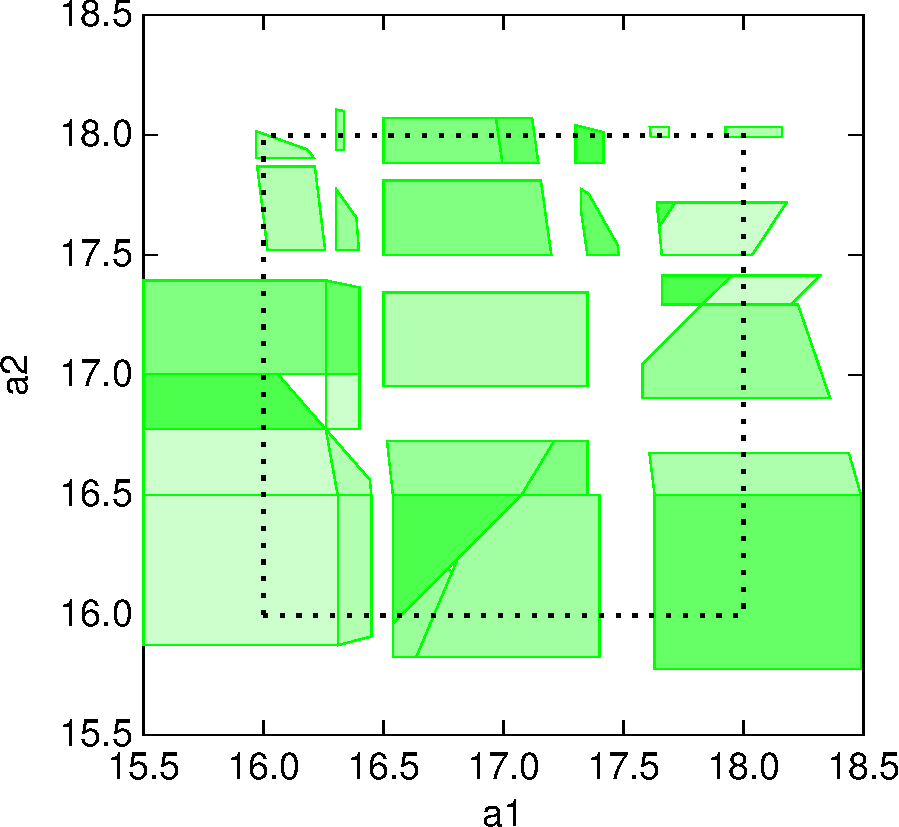
\includegraphics[width=0.6\textwidth]{rhb_cart2.pdf}
				\end{center}
			\end{column}
			\begin{column}{0.5\textwidth}
				\begin{center}
					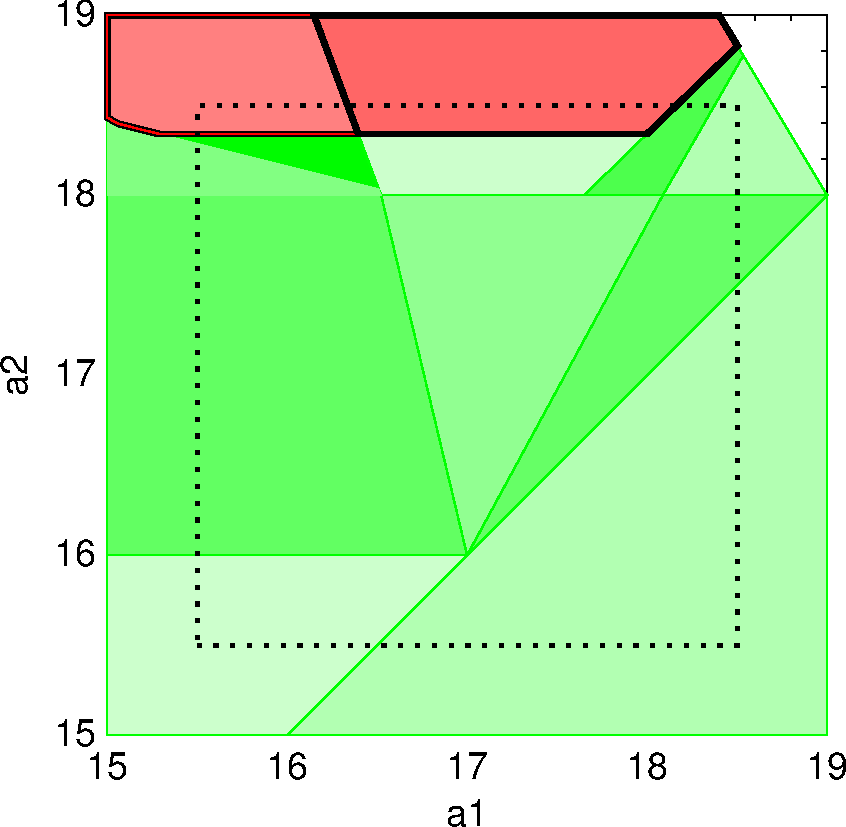
\includegraphics[width=0.6\textwidth]{good-bad.pdf}
				\end{center}
			\end{column}
		\end{columns}
		\end{itemize}

	\item \coulitem{Implementation}  \refer{AK12}
	\begin{itemize}
		\item Implemented in OCaml, using the Parma Polyhedra Library %PPL~\refer{bhz08}
	\end{itemize}
\end{itemize}

\end{block}    
%%%%%%%%%%%%%%%%%%%%%%%%%%%%%%%%%%%%%%%%%%%%%%%%%%%%%%%%%%%%




%%%%%%%%%%%%%%%%%%%%%%%%%%%%%%%%%%%%%%%%%%%%%%%%%%%%%%%%%%%%
\begin{block}{Try it!}

\begin{itemize}
	\item Distributed under the GNU General Public License
	\item \url{www.lsv.ens-cachan.fr/Software/hymitator/}
\end{itemize}

\end{block}
%%%%%%%%%%%%%%%%%%%%%%%%%%%%%%%%%%%%%%%%%%%%%%%%%%%%%%%%%%%%


%%%%%%%%%%%%%%%%%%%%%%%%%%%%%%%%%%%%%%%%%%%%%%%%%%%%%%%%%%%%
\begin{block}{References}
	\footnotesize
	%%%%%%%%%%%%%%%%%%%%%%%%%%%%%%%%%%%%%%%%%%%%%%%%%%%%%%%%%%%%
	%%%%%%%%%%%%%%%%%%%%%%%%%%%%%%%%%%%%%%%%%%%%%%%%%%%%%%%%%%%%
	%%%%%%%%%%%%%%%%%%%%%%%%%%%%%%%%%%%%%%%%%%%%%%%%%%%%%%%%%%%%
	\bibliographystyle{apalike} % abbrv alpha plain
	\bibliography{../biblioFM}
	%%%%%%%%%%%%%%%%%%%%%%%%%%%%%%%%%%%%%%%%%%%%%%%%%%%%%%%%%%%%
	%%%%%%%%%%%%%%%%%%%%%%%%%%%%%%%%%%%%%%%%%%%%%%%%%%%%%%%%%%%%
	%%%%%%%%%%%%%%%%%%%%%%%%%%%%%%%%%%%%%%%%%%%%%%%%%%%%%%%%%%%%
\end{block}    
%%%%%%%%%%%%%%%%%%%%%%%%%%%%%%%%%%%%%%%%%%%%%%%%%%%%%%%%%%%%


\vfill


\end{column}
%%%%%%%%%%%%%%%%%%%%%%%%%%%%%%%%%%%%%%%%%%%%%%%%%%

% \vfill

\end{columns}
%%%%%%%%%%%%%%%%%%%%%%%%%%%%%%%%%%%%%%%%%%%%%%%%%%
%%%%%%%%%%%%%%%%%%%%%%%%%%%%%%%%%%%%%%%%%%%%%%%%%%

\vfill

\end{frame}



\end{document}

